\documentclass[conference,a4paper]{IEEEtran}
% IEEE conference-style working manuscript. A4 supports the course's page budget.
\usepackage{cite}
\usepackage{amsmath,amssymb}
\usepackage{graphicx}
\usepackage{booktabs}
\usepackage{array}
\usepackage{placeins}
\usepackage{capt-of}
\usepackage[hidelinks]{hyperref}
\graphicspath{{figures/}}
\hyphenation{trans-crip-tomic re-pro-duc-ibil-ity}
\begin{document}
\title{Benchmarking Transcriptomic Feature Selection for Cross-Cohort Predictive Performance and Biomarker Reproducibility}
\author{\IEEEauthorblockN{Abbas El-Hajj Youssef \quad Jad Mcheik}
\IEEEauthorblockA{Department of Computer Science, American University of Beirut\\
Beirut, Lebanon\\
\href{mailto:aae145@mail.aub.edu}{aae145@mail.aub.edu} \quad
\href{mailto:jmm60@mail.aub.edu}{jmm60@mail.aub.edu}}}
\maketitle
\begin{abstract}
RNA-sequencing classifiers may predict Crohn's disease (CD) across cohorts while selecting inconsistent genes. We evaluated LASSO, Elastic Net, complementary-pairs Stability Selection, StableMate and TENTACLES using 689 intestinal tissue samples (495 CD, 194 \emph{Not IBD}) in four analytical cohorts and 9,983 shared genes. Each cohort was tested once after gene selection on the other three; a fixed class-balanced logistic classifier evaluated all selected panels. We separately measured gene overlap, gene-count sensitivity and Reactome pathway enrichment. Mean held-out AUROC ranged from 0.628 (Stability Selection) to 0.723 (corrected TENTACLES six-of-nine consensus). TENTACLES and LASSO had similar mean leave-one-cohort-out (LOCO) gene Jaccard similarity (0.210 and 0.211) despite different mean panel sizes (76.5 versus 281.5 genes); Elastic Net achieved AUROC 0.712 with Jaccard 0.115. TENTACLES produced significantly enriched Reactome pathways in three of four folds, but overlap from LOCO fits is not independent replication because training sets share cohorts. Differences in tissue, class balance and control populations further restrict interpretation. Predictive transfer and gene-selection consistency should be assessed jointly without treating either as proof of clinically validated biomarkers.
\end{abstract}
\begin{IEEEkeywords}
Crohn's disease, RNA sequencing, feature selection, cross-cohort validation, biomarker reproducibility
\end{IEEEkeywords}
% V2 numerical output independently audited from user-provided private export; see verification audit.
\section{Introduction}
\label{sec:introduction}
Crohn's disease (CD) is a chronic inflammatory disorder of the gastrointestinal tract with substantial variation among patients \cite{torres2017crohn}. RNA sequencing (RNA-seq) measures RNA abundance in tissue samples and provides expression estimates for thousands of genes \cite{conesa2016survey}. Comparing intestinal expression profiles from patients with CD and comparison groups can reveal disease-associated patterns that may inform biomarker research \cite{montesi2026tentacles}. These associations do not, by themselves, establish causation or clinical usefulness.

Machine-learning classifiers can use expression measurements to distinguish CD from \emph{Not IBD} samples. Yet the number of genes typically exceeds the number of patients, and many genes are correlated. Feature selection therefore narrows the measurements to a \emph{gene signature}: a subset used for prediction or subsequent biological analysis. This creates two separate questions. \emph{Predictive generalisation} asks whether a model correctly classifies samples from a cohort excluded from training. \emph{Gene-signature reproducibility} asks whether fitting a comparable selection procedure separately to different patient cohorts yields similar gene lists. A model can generalise while selecting different genes from one dataset to another.

For example, two correlated genes may carry similar predictive information, so a selection method can retain either one depending on the patients analysed. Ein-Dor \emph{et al.} found markedly different yet similarly predictive signatures in breast cancer expression data \cite{eindor2005outcome}; related work showed that reliable agreement could require much larger discovery samples \cite{eindor2006thousands}. These studies motivate measuring gene agreement separately from prediction. Agreement is not proof of a causal biomarker, and its magnitude also depends on signature size.

Cohorts introduce further variation through differences in tissue composition, patient populations, sequencing protocols and class balance. Random train--test splits within one study can preserve such study-specific characteristics in both partitions. Cross-study evaluation instead tests models on cohorts not used for development \cite{bernau2014cross}. We use leave-one-cohort-out (LOCO) evaluation, training on three cohorts and testing on the fourth in turn. Importantly, gene lists selected in different LOCO rounds are \emph{not} independent discoveries: their training sets overlap. We therefore distinguish their descriptive agreement from signatures fitted separately within individual cohorts.

Existing approaches differ in what they try to stabilise. LASSO selects genes through sparse regression coefficients \cite{tibshirani1996lasso}; Elastic Net also accommodates correlated predictors \cite{zou2005elastic}. Stability Selection favours genes repeatedly selected from subsamples \cite{meinshausen2010stability}, whereas StableMate targets predictors whose associations remain comparatively stable across environments \cite{deng2024stablemate}. TENTACLES combines feature-importance evidence from several learning algorithms into a consensus panel \cite{montesi2026tentacles}. Selection frequency, between-environment stability and agreement between algorithms are distinct properties; none alone guarantees replication across independent cohorts.

TENTACLES has already studied this Crohn's disease collection and compared biomarker-selection approaches \cite{montesi2026tentacles}. We instead examine how \emph{predictive transfer} relates to \emph{gene-set consistency} across LASSO, Elastic Net, Stability Selection, StableMate and TENTACLES. Our four analytical cohorts contain 689 samples from six BioProjects and share 9,983 genes. Alongside method-specific predictions, a fixed downstream classifier assesses the selected gene panels under common prediction settings. We compare gene overlap across LOCO fits, examine signature-size effects and assess Reactome pathway agreement. Because the LOCO training sets overlap, agreement among their selected genes does not demonstrate independent biomarker replication.

\section{Materials and Methods}
\subsection{Data sources and cohort characteristics}
\label{sec:dataset}
We used the processed intestinal tissue RNA-seq count matrices compiled for TENTACLES \cite{montesi2026tentacles}; we did not reprocess raw sequencing reads. The collection contains 689 samples labelled CD (495) or \emph{Not IBD} (194), grouped into four analytical cohorts from six BioProjects (Table~\ref{tab:cohorts}). The comparison label is retained from the source data, but does not imply that every control was a healthy volunteer. For instance, D3 includes non-tumour intestinal tissue from colorectal-cancer surgery \cite{friedrich2021il1}.

\begin{table}[!t]
\caption{Cohort composition by source BioProject.}
\label{tab:cohorts}
\centering\footnotesize
\setlength{\tabcolsep}{3.5pt}
\renewcommand{\arraystretch}{1.1}
\begin{tabular}{@{}llrrr@{}}
\toprule
Cohort & BioProject(s) & $n$ & CD & Not IBD\\
\midrule
D1 & PRJNA248469 & 260 & 218 & 42\\
D2 & \shortstack[l]{PRJNA565216\\PRJNA985602} & 179 & 134 & 45\\
D3 & PRJNA702434 & 76 & 34 & 42\\
D4 & \shortstack[l]{PRJNA728646\\PRJNA961704} & 174 & 109 & 65\\
\midrule
Total & Six BioProjects & 689 & 495 & 194\\
\bottomrule
\end{tabular}
\end{table}

The CD fraction ranges from 44.7\% (D3) to 83.8\% (D1), and median assigned counts across common genes range from 1.78 to 12.01 million per sample. The cohorts also differ in tissue site: D1 comprises ileal biopsies; D2 includes ileal and colonic biopsies; D3 includes small- and large-intestinal samples; and D4 does not provide tissue-site labels in the supplied metadata. Source count CSVs lacked sample identifiers and had 670 rows ordered differently from their metadata. We recovered the IDs from accompanying R data files, aligned expression rows to metadata and verified the original counts and labels without changing their values. The original matrices contained 10,061 genes for D1--D3 and 41,257 for D4; the shared gene-name intersection contained 9,983 genes.

Seven D3 records carried exclusion flags from the source study's quality-control assessment \cite{friedrich2021il1}. They were retained to match the published 76-sample D3 cohort; their inclusion remains a limitation. Exploratory principal-component analysis (PCA) shows cohort-associated expression structure (Fig.~\ref{fig:pca}). It does not establish whether the differences are technical or biological and was not used to train models.

\begin{figure}[!t]
\centering
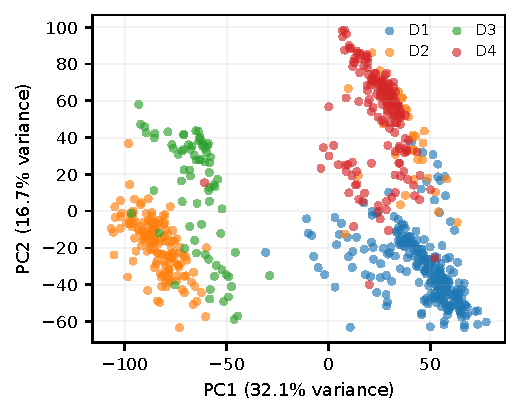
\includegraphics[width=\columnwidth]{cohort_pca_ieee.pdf}
\caption{Exploratory PCA of $\log_2(1+\mathrm{CPM})$ expression across shared genes, coloured by cohort. This descriptive visualisation was not used in model fitting.}
\label{fig:pca}
\end{figure}

\subsection{Cross-cohort evaluation}
\label{sec:evaluation_design}
Each LOCO round held out one analytical cohort and used the other three for model development (Table~\ref{tab:splits}). Saved sample assignments confirmed no train/test overlap within a round. Some cohorts comprise multiple BioProjects, so this is cohort-level rather than six-study-level validation.

\begin{table}[!t]
\caption{Outer LOCO assignments. Each held-out cohort is never used for its own gene selection or model training.}
\label{tab:splits}
\centering\footnotesize
\begin{tabular}{@{}lrrl@{}}
\toprule
Test cohort & Train $n$ & Test $n$ & Development cohorts\\
\midrule
D1 & 429 & 260 & D2, D3, D4\\
D2 & 510 & 179 & D1, D3, D4\\
D3 & 613 & 76 & D1, D2, D4\\
D4 & 515 & 174 & D1, D2, D3\\
\bottomrule
\end{tabular}
\end{table}

LASSO and Elastic Net tuned regularisation using three inner cohort-held-out validation splits within each development set, selecting settings by mean validation AUROC. Other methods retained their method-specific selection and tuning procedures. In the sparse logistic pipelines, expression was transformed to $\log_2(1+\mathrm{CPM})$, where CPM used counts summed over the shared genes in each sample. Genes with CPM $>1$ in at least 10\% of the fitting samples and nonzero variance were retained. Gene filtering and standardisation were fitted only on each relevant training partition and then applied to validation or test data. Native methods used their own documented preprocessing. Method-specific prediction outputs were retained separately and are not treated as matched classifier comparisons.

\subsection{Controlled downstream classifier}
\label{sec:common_classifier}
To compare the predictive usefulness of selected genes under the same downstream model, we used each method's frozen, outer-training-selected panel in a separate L2-regularised logistic regression. Panels comprised the nonzero sparse-model coefficients, Stability Selection genes at a 0.60 frequency cutoff, native StableMate stable-significant genes, and the TENTACLES consensus. All panels were evaluated on the same four LOCO splits, with $\log_2(1+\mathrm{CPM})$ expression, training-only standardisation and class-balanced fitting (scikit-learn \texttt{liblinear}, $C=1$, 5,000 maximum iterations, seed 123). CD was positive; probabilities of at least 0.5 were classified as CD. The learner and evaluation settings were fixed, but the upstream feature selection, tuning and gene counts differed.

\subsection{Prediction measures}
\label{sec:predictive_metrics}
CD was the positive class for the verified Python prediction pipelines. We report AUROC and balanced accuracy (mean sensitivity and specificity), which helps describe performance despite differing CD prevalence. Threshold-based measures used a CD probability threshold of 0.5; F1-score and average precision are reported where available. Each cohort's result is shown separately, with an unweighted four-cohort mean and, where available, the standard deviation across cohorts.

Within-cohort stratified bootstrap intervals for AUROC used 1,000 resamples for LASSO/Elastic Net and 2,000 for StableMate. These intervals reflect test-sample variation conditional on the fitted models; they do not estimate uncertainty over future independent cohorts.

\subsection{Gene and pathway agreement}
\label{sec:reproducibility_metrics}
Let $S_{m,f}$ denote the genes selected by method $m$ when cohort $f$ is held out. For each method, we calculated the Jaccard similarity between all six unordered pairs of its four LOCO signatures and averaged them:
\begin{equation}
\bar{J}_m=\frac{1}{6}\sum_{a<b}
\frac{|S_{m,a}\cap S_{m,b}|}{|S_{m,a}\cup S_{m,b}|}.
\label{eq:jaccard}
\end{equation}
We also report panel sizes and the number of genes appearing in all four panels. LOCO training sets overlap in two cohorts, so the six pairwise scores are dependent measures of \emph{selection consistency}, not six independent replications. Signatures selected separately within single cohorts provide a distinct comparison where available.

Because Jaccard similarity depends partly on gene-set size, we additionally compared the four highest-ranked genes within each LOCO panel for LASSO, Elastic Net, Stability Selection and StableMate. Rankings used absolute standardised coefficients, subsample selection frequency, and native predictive importance, respectively; ties were settled by gene name. Four genes were the largest common panel size available across these four methods and folds. An exploratory top-ten comparison covered only LASSO, Elastic Net and StableMate. TENTACLES V2 was excluded from the fixed top-four analysis: its genuine vote counts provide coarse evidence of importance but leave many ties among six- to nine-vote genes, so a unique meaningful within-panel top-four ordering is not available. These truncated-panel comparisons assess selection overlap, not newly fitted classifiers.

For the five methods' LOCO-selected panels, Reactome v98 pathways \cite{ragueneau2026reactome} were tested for over-representation against the eligible training-gene background. We used one-sided hypergeometric tests for pathways containing 10--500 eligible genes, followed by Benjamini--Hochberg correction ($q<0.05$) \cite{benjamini1995fdr}. Pathway Jaccard similarity compared sets of significant pathways; it was undefined when both sets were empty. Pathway overlap remains descriptive because the discovery sets overlap, and enrichment power depends on panel size and gene annotation coverage.

\subsection{LASSO and Elastic Net}
\label{sec:sparse_methods}
We used logistic-regression versions of LASSO and Elastic Net as sparse predictive baselines \cite{tibshirani1996lasso,zou2005elastic}. Both minimise a class-weighted logistic loss with a penalty on the gene coefficients $\boldsymbol{\beta}$ of the form
\begin{equation}
\Omega(\boldsymbol{\beta})=\alpha\lVert\boldsymbol{\beta}\rVert_1+
\frac{1-\alpha}{2}\lVert\boldsymbol{\beta}\rVert_2^2.
\label{eq:sparse_penalty}
\end{equation}
LASSO uses $\alpha=1$, whereas Elastic Net allows a mixture of $L_1$ and $L_2$ regularisation. Models were fitted using scikit-learn's SAGA solver with balanced class weights, at most 1,600 iterations, tolerance $10^{-3}$ and random seed 355. The inverse regularisation strength was searched over $C\in\{0.001,0.01,0.1,1\}$; Elastic Net additionally searched $\alpha\in\{0.5,0.9\}$.

For each outer LOCO split, we chose $(C,\alpha)$ using the mean AUROC across three inner cohort-held-out validation splits. Ties favoured smaller $C$, then larger $\alpha$. After refitting on all three development cohorts, genes with absolute standardised-model coefficients exceeding $10^{-8}$ formed the selected signature. The final model also predicted the untouched outer test cohort. Preprocessing was refitted within every inner training split as described in Section~\ref{sec:evaluation_design}; no fixed number of genes was imposed.

To evaluate gene agreement between independently analysed cohorts, we separately fitted LASSO and Elastic Net within each cohort. Here, hyperparameters were selected by stratified three-fold cross-validation within that cohort, followed by a fit on all its samples. We also recorded selection frequencies from 30 stratified half-sample refits per cohort and method as an exploratory sensitivity measure; these frequencies were not the formal Stability Selection procedure described separately. Within-cohort signatures were compared with each other, but their training-set predictions were not reported as external test results.

\subsection{Stability Selection}
\label{sec:stability_method}
We implemented complementary-pairs Stability Selection using a class-balanced $L_1$-logistic base model \cite{meinshausen2010stability}. Within each training set, 30 random partitions produced 60 complementary half-sample fits. The base model's regularisation strength was calibrated on training data to select approximately 50 genes per fit. Each gene's selection frequency was its number of selections divided by 60. We saved signatures at frequency cutoffs 0.60, 0.75 and 0.90, with 0.75 designated as the original procedure's primary cutoff. The controlled five-method comparison instead uses the 0.60 panels; these choices must not be conflated. The method-specific predictive pipeline used the 50 highest-frequency genes with nonzero selection frequency and a fixed class-balanced $L_2$-logistic classifier ($C=1$), which is distinct from any thresholded signature. We also computed signatures within each individual cohort for separate gene-agreement analysis. This is an implementation of complementary-pairs selection frequencies, not the authors' \texttt{stabs} package; its theoretical false-selection bound was not claimed because the required assumptions were not established.

\subsection{StableMate}
\label{sec:stablemate_method}
We used the authors' \texttt{StableMate} R package (version 0.1.0, pinned revision) \cite{deng2024stablemate}. For each LOCO fit, the three development cohorts defined the environments. The native procedure combined a random LASSO prefilter of 50 predictors per candidate, 2,000 candidate models in each of the prediction and stability ensembles, and 1,000 bootstrap replicates for importance estimation. A gene entered the stable-significant panel only if both its predictive and stability significance scores exceeded 0.975. Native held-out predictions used the fitted StableMate logistic predictor; these were kept separate from the controlled-classifier experiment, which refitted the same fixed $L_2$ learner to the selected panel. All four native fits and numerical prediction exports were audited, although the saved native R objects were not independently retrained and their reported fitting warnings were not resolved by that audit.

\subsection{TENTACLES consensus procedure}
\label{sec:tentacles_method}
We used the authors' \texttt{TENTACLES} R package (version 0.1.0, pinned revision) \cite{montesi2026tentacles} as an algorithm-consensus selector. On each LOCO development set, the native RNA-seq preprocessing was followed by ten classifier--selector pairs: random forest/correlation, MLP/ROC, bagged MLP/ROC, linear SVM/Boruta, C5 rules/Boruta, LightGBM/ROC, decision tree/Boruta, MARS/Boruta, XGBoost/base, and PLS/Boruta. The classifiers were tuned with five-fold cross-validation, five candidate settings and F1 as the target metric; class downsampling was enabled. The corrected protocol explicitly preserves CD as the positive event and checks that the native fitted F1 scores use that orientation. The primary consensus requires at least six votes among nine models after excluding XGBoost; five of nine is a sensitivity threshold. Native votes must reproduce the exported gene sets. Only training cohorts contribute to native selection; a subsequent fixed logistic classifier supplies external predictions, not the package's internally fitted \texttt{testConsensus} model. The four native fits and both external evaluations have completed locally; the saved reports document D3/D4 recovery and incomplete tuning for the excluded D4 XGBoost model. The exported four-fold gene lists and 689 held-out predictions were independently checked against native voting records and saved scores; this check did not retrain the native R models or resolve their fitting warnings.

\begin{table}[!t]
\caption{Selected-gene panels used by the common classifier.}
\label{tab:method_overview}
\centering\footnotesize
\setlength{\tabcolsep}{3pt}
\renewcommand{\arraystretch}{1.13}
\begin{tabular}{@{}p{2.0cm}p{5.9cm}@{}}
\toprule
Method & Panel definition \\
\midrule
LASSO & Nonzero logistic coefficients ($|\beta|>10^{-8}$) \\
Elastic Net & Nonzero logistic coefficients ($|\beta|>10^{-8}$) \\
Stability Selection & Frequency $\geq0.60$; original primary cutoff $0.75$ \\
StableMate & Predictive and stability significance each $>0.975$ \\
TENTACLES & V2 consensus: at least 6 votes among 9 eligible models; verified by independent panel/vote checks \\
\bottomrule
\end{tabular}
\end{table}

\section{Results}
\label{sec:results}
\subsection{Prediction on excluded cohorts}
\label{sec:results_prediction}
Under the same downstream logistic classifier, four-cohort mean AUROC ranged from 0.628 (Stability Selection) to 0.723 (TENTACLES V2); the mean balanced-accuracy range was 0.563--0.655 (Table~\ref{tab:results_main}). TENTACLES had the highest observed mean AUROC, followed by Elastic Net (0.712), but the difference between these means was only 0.011. These comparisons describe the four observed cohorts, not a tested superiority claim.

\begin{table*}[!t]
\caption{Controlled five-method benchmark. Every selected gene panel was evaluated with class-balanced $L_2$ logistic regression ($C=1$) on the same four LOCO train/test splits; CD is the positive class. AUROC and BA (balanced accuracy) are unweighted four-cohort means, with between-cohort sample SD for AUROC. Mean gene-set Jaccard averages six dependent LOCO panel pairs; ``all four'' counts genes present in every panel. Panel size varies by selector and is not matched in this primary comparison.}
\label{tab:results_main}
\centering\footnotesize
\setlength{\tabcolsep}{5.4pt}
\renewcommand{\arraystretch}{1.18}
\begin{tabular}{@{}lccccc@{}}
\toprule
Selector & AUROC mean (SD) & BA mean & Gene panel mean [min--max] & LOCO $\bar J$ & Genes in all 4\\
\midrule
LASSO & 0.689 (0.135) & 0.619 & 281.5 [271--295] & 0.211 & 36\\
Elastic Net & 0.712 (0.105) & 0.628 & 352.5 [39--671] & 0.115 & 6\\
Stability Selection ($\pi\geq0.60$) & 0.628 (0.051) & 0.563 & 6.3 [4--9] & 0.128 & 0\\
StableMate & 0.659 (0.083) & 0.598 & 15.8 [14--20] & 0.033 & 0\\
\textbf{TENTACLES V2 (6/9)} & \textbf{0.723 (0.100)} & \textbf{0.655} & 76.5 [61--91] & 0.210 & 6\\
\bottomrule
\end{tabular}
\end{table*}

\begin{figure*}[!t]
\centering
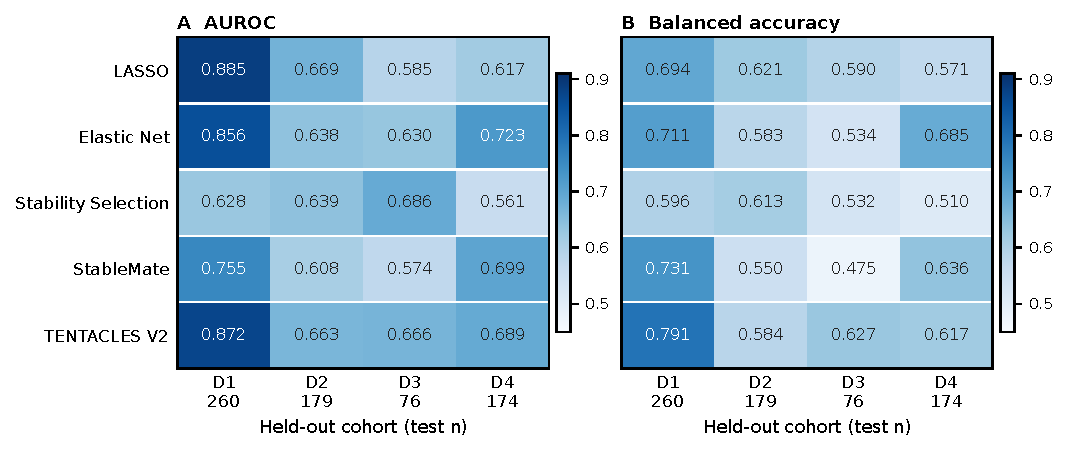
\includegraphics[width=\textwidth]{heldout_metric_heatmaps.pdf}
\caption{External test performance of all five gene-panel selectors, separately for each left-out cohort. Both panels use the same fixed, class-balanced logistic classifier ($C=1$), fitted and scaled on the other three cohorts. Entries show (A) area under the receiver-operating-characteristic curve (AUROC) and (B) balanced accuracy, equal to the mean of CD sensitivity and \emph{Not IBD} specificity at probability threshold 0.5. Cohort sample counts are given below D1--D4; darker cells indicate higher values. The same test patients are used for all methods within each column.}
\label{fig:results_heatmap}
\end{figure*}

Performance depended strongly on the held-out cohort (Fig.~\ref{fig:results_heatmap}). On D1, LASSO attained AUROC 0.885, whereas Stability Selection obtained 0.628. On D3, Stability Selection led with AUROC 0.686; on D4, Elastic Net led with 0.723. TENTACLES was not the best-scoring selector in every test cohort. AUROC and balanced accuracy could also disagree: Stability Selection reached AUROC 0.686 on D3 but balanced accuracy 0.532 at the fixed probability cutoff. The contrast is relevant because CD prevalence varied from 44.7\% in D3 to 83.8\% in D1.

\subsection{TENTACLES consensus-vote sensitivity}
\label{sec:results_tentacles}
The corrected TENTACLES workflow yielded primary six-of-nine consensus panels of 73, 91, 81 and 61 genes (D1--D4). All native exported votes matched these panels and all 689 held-out predictions matched their reported scores. The primary rule gave mean AUROC 0.723 and mean balanced accuracy 0.655. Relaxing the consensus to five votes selected 90--115 genes per fold and reduced mean AUROC to 0.691 (Table~\ref{tab:tentacles_sensitivity}). Six votes performed better on D1, D3 and D4, but not on D2; it should not be described as uniformly superior.

\begin{table}[!t]
\caption{TENTACLES V2 on each held-out cohort: prespecified 6/9-vote primary versus 5/9-vote sensitivity. AUROC intervals are 95\% patient-stratified bootstrap intervals (1,000 resamples), conditional on the fitted six-vote model; they do not quantify variability across new cohorts. BA is balanced accuracy.}
\label{tab:tentacles_sensitivity}
\centering\footnotesize
\setlength{\tabcolsep}{2.9pt}
\renewcommand{\arraystretch}{1.1}
\begin{tabular}{@{}lcccc@{}}
\toprule
Test & 6-vote genes & 6-vote AUROC [95\% CI] & 6-vote BA & 5-vote AUROC\\
\midrule
D1 & 73 & 0.872 [0.821, 0.918] & 0.791 & 0.824\\
D2 & 91 & 0.663 [0.569, 0.753] & 0.584 & 0.666\\
D3 & 81 & 0.666 [0.529, 0.796] & 0.627 & 0.647\\
D4 & 61 & 0.689 [0.608, 0.765] & 0.617 & 0.626\\
\midrule
Mean & 76.5 & 0.723 & 0.655 & 0.691\\
\bottomrule
\end{tabular}
\end{table}

D3 and D4 required documented recoveries of previously saved native fits rather than new fitting runs. D3 lacked XGBoost variable importance; D4 had only four selected cross-validation resamples for XGBoost. Both exceptions concern the model excluded from the prespecified nine-voter consensus. The other nine voters passed the saved orientation and feature-importance checks; native tuning warnings remain and are not erased by the successful downstream evaluation.

\subsection{Gene-panel agreement and size sensitivity}
\label{sec:results_genes}
The relationship between prediction and gene-set agreement was not monotonic (Fig.~\ref{fig:tradeoff}). LASSO and TENTACLES achieved similar mean LOCO Jaccard similarity (0.211 and 0.210), despite selecting on average 282 and 77 genes, respectively (Table~\ref{tab:results_main}). Elastic Net slightly exceeded LASSO's mean AUROC but had a lower mean gene Jaccard (0.115 versus 0.211). StableMate selected an average of 16 genes and had the lowest mean Jaccard (0.033). These values are sensitive to panel size and the shared cohorts in the LOCO training sets.

\begin{figure*}[!t]
\centering
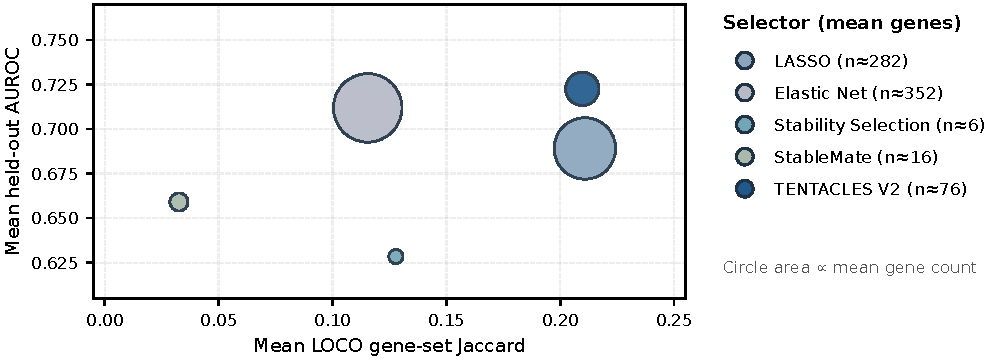
\includegraphics[width=0.92\textwidth]{prediction_vs_agreement.pdf}
\caption{Observed prediction--selection relationship for five methods. Each circle locates the four-cohort mean held-out AUROC versus the mean Jaccard of six pairs of overlapping-training LOCO gene lists. Circle area reflects mean panel size, and the legend identifies each method. The plot is descriptive; selection panel sizes and upstream procedures are not matched.}
\label{fig:tradeoff}
\vspace{1ex}
\begin{minipage}[t]{0.485\textwidth}
\centering
\captionof{table}{Independent-cohort sparse signatures. Gene counts are from models fitted separately within each cohort; mean $\bar J$ covers six patient-disjoint cohort pairs. These gene lists were not used in held-out prediction.}
\label{tab:independent_sizes}
\vspace{0.4ex}
\footnotesize
\setlength{\tabcolsep}{5pt}
\begin{tabular}{@{}lrrrrc@{}}
\toprule
Selector & D1 & D2 & D3 & D4 & $\bar J$\\
\midrule
LASSO & 2523 & 2119 & 1734 & 2623 & 0.164\\
Elastic Net & 2831 & 4025 & 1934 & 2905 & 0.209\\
\bottomrule
\end{tabular}
\end{minipage}\hfill
\begin{minipage}[t]{0.485\textwidth}
\centering
\captionof{table}{Reactome v98 enrichment in four LOCO training panels per method. D1--D4 are counts of pathways passing Benjamini--Hochberg $q<0.05$. $\bar J$ averages nonempty-union pathway-set pairs; n/a indicates all unions empty. Gene-panel sizes differ.}
\label{tab:results_pathways}
\vspace{0.4ex}
\footnotesize
\setlength{\tabcolsep}{4pt}
\begin{tabular}{@{}lccc@{}}
\toprule
Selector & D1/D2/D3/D4 & Folds & $\bar J$\\
\midrule
LASSO & 1/3/4/0 & 3/4 & 0.222\\
Elastic Net & 3/1/4/9 & 4/4 & 0.273\\
Stability Selection & 0/0/0/0 & 0/4 & n/a\\
StableMate & 0/0/0/0 & 0/4 & n/a\\
TENTACLES V2 & 0/11/8/9 & 3/4 & 0.256\\
\bottomrule
\end{tabular}
\end{minipage}
\vspace{2.0ex}
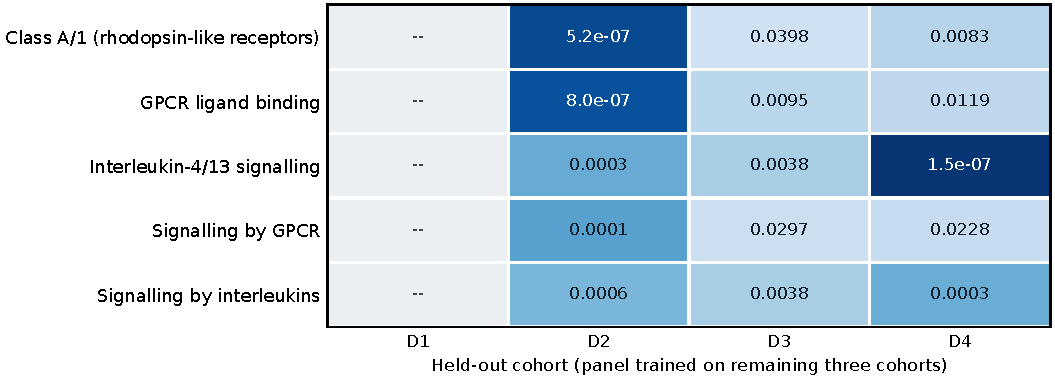
\includegraphics[width=0.88\textwidth]{tentacles_v2_reactome_terms.pdf}
\captionof{figure}{Recurring Reactome v98 terms in the TENTACLES V2 six-vote LOCO panels. Each cell shows the adjusted enrichment $q$ value when $q<0.05$; ``--'' indicates no significant term. These are descriptive overlaps because LOCO training cohorts and gene annotations overlap.}
\label{fig:v2_pathways}
\end{figure*}

Only six genes appeared in all four primary TENTACLES V2 panels: \textit{CLDN18}, \textit{FFAR2}, \textit{MMP3}, \textit{NOS2}, \textit{PAQR5} and \textit{PML}. These are repeated LOCO selections, not independently validated clinical markers. Each LOCO training pair shares two cohorts; consequently the six pairwise Jaccard measurements are dependent rather than six independent replications.

A four-gene, fixed-size sensitivity analysis was possible for LASSO, Elastic Net, Stability Selection and StableMate only: one stability-selection panel contained just four genes. Their respective mean top-four Jaccards were 0.103, 0, 0.103 and 0.048. The corresponding top-ten comparison, available only for LASSO, Elastic Net and StableMate, yielded 0.137, 0.037 and 0.035. TENTACLES V2 supplies genuine vote counts but many equal-count ties, making its top-four ordering arbitrary without a further prespecified rule. Thus the four-method size-matched result cannot be presented as a five-method test. Fixing $K$ also changes the target from agreement of the full selected panel to agreement among a few highest-ranked genes.

To examine gene overlap from patient-disjoint discovery groups, we also fitted LASSO and Elastic Net separately within each cohort. The resulting gene sets were much larger than their LOCO counterparts (Table~\ref{tab:independent_sizes}); mean pairwise Jaccard was 0.164 for LASSO and 0.209 for Elastic Net. Their sizes make these values hard to interpret as evidence of selective, reproducible biomarkers, despite the nonoverlapping patients.


\subsection{Reactome pathway overlap}
\label{sec:results_pathways}
Across the five LOCO panel types, the number of significantly over-represented Reactome pathways varied sharply (Table~\ref{tab:results_pathways}). TENTACLES V2 yielded 0, 11, 8 and 9 significant pathways across D1--D4, with mean pairwise significant-pathway Jaccard 0.256. Elastic Net yielded 3, 1, 4 and 9 pathways ($\bar J=0.273$), and LASSO yielded 1, 3, 4 and 0 ($\bar J=0.222$). No fold of Stability Selection or StableMate produced FDR-significant pathways; their Jaccard similarities are therefore undefined because every compared pathway set is empty, not because the overlap equals zero.


In the V2 panels, interleukin signalling, interleukin-4/interleukin-13 signalling and several G-protein-coupled receptor pathways appeared as significantly enriched terms in D2, D3 and D4 (Fig.~\ref{fig:v2_pathways}). No TENTACLES pathway survived FDR correction in D1. Enrichment reflects over-representation of selected genes against each fold's eligible-gene background, not differential expression, biological causation or independent pathway replication.





\section{Discussion}
\label{sec:discussion}
\subsection{Predictive transfer and gene-list consistency are distinct}
\label{sec:discussion_tradeoff}
This study tested whether feature-selection strategies that predict CD in an unseen cohort also return consistent gene lists. Under a fixed logistic classifier, TENTACLES V2 had the highest observed mean AUROC (0.723), but the method leading on AUROC changed across D1--D4. The cohort-specific results indicate substantial heterogeneity, and a 0.011 difference between TENTACLES and Elastic Net in four-cohort mean AUROC does not establish that either is generally superior. Patient-stratified bootstrap intervals quantify sampling variability within each test cohort, not uncertainty about deployment to new cohorts.

Gene agreement told a different story. LASSO and TENTACLES produced nearly identical mean LOCO Jaccards (0.211 and 0.210) with markedly different panel sizes; Elastic Net had higher predictive AUROC than LASSO but lower gene Jaccard. Thus neither model performance nor panel size alone determines agreement. Correlated predictors may substitute for one another, while regularisation strength and method-specific selection objectives can change signature sizes. The controlled downstream predictor holds the classifier and test partitions constant, but the upstream tuning procedures, preprocessing and number of genes still vary, so differences cannot be attributed causally to the selector alone.

\subsection{What reproducibility can be inferred?}
\label{sec:discussion_reproducibility}
The six Jaccard comparisons per method were calculated between LOCO fits that share two of their three training cohorts. They therefore quantify how sensitive each selector is to which cohort was excluded, rather than providing four independent discovery replications. Indeed, the separate LASSO and Elastic Net analyses fitted to patient-disjoint cohorts selected thousands of genes and showed substantial size-dependent overlap, illustrating why raw Jaccard is not sufficient to identify stable, selective clinical markers. The fixed top-four analysis partly controls signature length but covers only four selectors and uses method-specific importance rankings; small lists are especially sensitive to ties and individual genes. Native TENTACLES votes have many ties, so an arbitrary top-four vote ranking would not produce a defensible five-method fairness result.

TENTACLES selected six genes in every LOCO fit, including \textit{NOS2} and \textit{CLDN18}, but repeated selection from overlapping training sets is not a clinical validation of any of them. Confirming a candidate biomarker would require a separately collected clinical cohort, consistent control definitions and direct assessment of diagnostic value.

\subsection{Pathway-level patterns are conditional on panel size}
\label{sec:discussion_pathway}
Pathway enrichment sometimes revealed more recurring terms than exact gene-list overlap. In particular, the corrected TENTACLES V2 panels showed recurring interleukin and GPCR-related annotations across D2--D4, while its D1 panel had none passing FDR correction. Elastic Net produced significant terms in all four folds, yet the significant-pathway Jaccard remained moderate (0.273). This does not establish that pathways are universally more reproducible than genes: pathway terms are correlated, the tests use highly unequal gene panels and large panels often have greater statistical power. Stability Selection and StableMate's lack of significant enriched pathways may reflect their 4--20-gene signatures, not the absence of relevant biology. An empty union of significant pathways yields an undefined Jaccard, not evidence of either perfect consistency or zero biological similarity.

\subsection{Cohort composition and implementation limitations}
\label{sec:discussion_limits}
The four analytical cohorts draw on six BioProjects, not six separate holdouts. They vary in CD prevalence, intestinal tissue site, comparison-group composition and assigned count totals. D3 comparison tissue came from colorectal-cancer surgery; tissue site is missing from the supplied D4 metadata. Gene expression may therefore encode non-disease differences that transfer unevenly between cohorts. Descriptive PCA shows cohort structure but cannot distinguish true biological shifts from technical batch effects. We did not apply post-hoc batch correction using the held-out cohorts.

Seven D3 source records had an exclusion flag. Retaining them preserves the published TENTACLES four-cohort collection, but leaves an unperformed QC-exclusion sensitivity analysis. The original RNA-seq reads and clinical diagnoses were not re-audited; only the supplied count tables, metadata alignment, signatures and evaluation outputs were checked.

The V2 output archive independently reproduced the selected nine-voter consensus lists, AUROC, balanced accuracy, and patient-level predictions, and the fixed logistic predictor could be refitted to reproduce V2 probabilities within numerical tolerance. This is not equivalent to independently rerunning all ten author-native classifiers from their original large R objects. The saved D3 and D4 recoveries preserved the fitted models and excluded XGBoost from consensus as prespecified; D4 XGBoost had only four selected cross-validation resamples. Warnings involving native MLP, Boruta and LightGBM candidates were recorded but were not proven harmless. We consequently interpret the nine-voter panel results as an audited adaptation of TENTACLES, not an exact replication of the original publication or proof that every native tuning candidate succeeded.

\subsection{Implications}
\label{sec:discussion_implications}
Transcriptomic benchmark reports should give held-out performance by source cohort alongside the size and overlap of selected signatures, rather than publishing a single mean accuracy or one consensus gene list. Repeating the experiment in independent, tissue-matched cohorts, testing prespecified panel sizes and sensitivity to D3's exclusion flags would better separate biological reproducibility from training-set dependence. Within this four-cohort benchmark, the results support an empirical comparison of candidate panels, but not a clinically validated biomarker claim.

\section{Conclusion}
\label{sec:conclusion}
Across 689 intestinal RNA-seq samples, five selection strategies gave cohort-dependent predictive performance under the same downstream classifier and markedly different gene panels. The highest observed mean AUROC (0.723, TENTACLES V2) did not imply uniformly superior performance or independent biomarker reproducibility. Gene-set overlap and Reactome enrichment also depended on overlapping discovery sets, panel size and source-cohort differences. Cross-cohort prediction, selection consistency and biological validation should therefore be reported and interpreted as distinct outcomes.

\section*{Code and Data Availability}
The project repository is at \url{https://github.com/abbaselhajj/CMPS355-Transcriptomic-Feature-Selection}. Source RNA-seq data are described in the cited studies; reproducibility scripts and aggregate results are being deposited in the repository.

\section*{Acknowledgment}
AI-assisted tools supported computational scripting, numerical checks, visualization and editorial refinement. The authors take responsibility for the reported methods, results and interpretations.

\bibliographystyle{IEEEtran}
\bibliography{references}
\end{document}
